%\documentclass[a4paper,10pt]{article}
\documentclass[10pt]{article}
\usepackage[utf8]{inputenc}
\usepackage{xspace}
\usepackage{url}
\usepackage{graphicx,graphics} 
\usepackage{color}
\usepackage{amsmath}
\usepackage{amsfonts}
\usepackage{amssymb}
\usepackage{amsthm}
\usepackage{algorithm}
\usepackage{algorithmic}
\usepackage{longtable}
\usepackage{complexity}
\usepackage{tkz-graph}
\usepackage{float}
\usepackage{tabularx}
\usepackage{setspace}
\usepackage{icomma}
\renewcommand{\algorithmicrequire}{\textbf{Input:}}
\renewcommand{\algorithmicensure}{\textbf{Output:}}
\usepackage{authblk}
\usepackage[colorlinks=true,breaklinks=true,linkcolor=blue]{hyperref}


\newcommand\rmatching{${\cal R}$-matching\xspace}
\newcommand\mdelay{$\cal M$-delay\xspace}
\newcommand\matchedgraph{{\bf matched graph}}
\newtheorem{proposition}{Proposition}
\newtheorem{theorem}{Theorem}

\setlength{\parskip}{1ex} % Espace entre les paragraphes

\newtheorem{fact}{Fact}
\newtheorem{lemma}[theorem]{Lemma}
\newtheorem{definition}{Definition}
\newtheorem{corollary}{Corollary}

% \renewcommand{\thefootnote}{\*}

\newcommand{\todo}[1]{{\color{red} TODO: {#1}}}
\newcommand\pazl{\textsc{pazl}\xspace}
\newcommand\pall{\textsc{pall}\xspace}
\newcommand\bra{\textsc{bra}\xspace}
\newcommand\pra{\textsc{pra}\xspace}
\newcommand\minpra{\textsc{min-pra}\xspace}
%opening
\title{Deterministic Scheduling of Periodic Messages for Cloud RAN}
 

\author[1]{Dominique Barth}
\author[1,2]{Ma\"el Guiraud}
% \author[1]{Christian Cad\'er\'e}
 \author[2]{Brice Leclerc}
 \author[2]{Olivier Marc\'e}
\author[1]{Yann Strozecki}
\affil[1]{David Laboratory, UVSQ}
\affil[2]{Nokia Bell Labs France}

\begin{document}

\begin{section}{Implementation details}
\begin{subsection}{Model of the generated graphs}
The graphs we study in are some two levels trees. First of all, two parameters set up the number of each node (contention point) at each level of the tree. The first level of the tree models the datacenters, and the second level of the trees models the switches in the core of the network.
Here is an example of a tree generated with 2  nodes of level 1 and 4  node of level 2.

\begin{center}
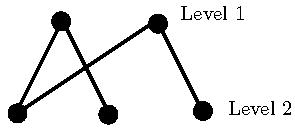
\includegraphics[width=0.5\textwidth]{random23}
\end{center}

This architecture models a real topology which can correspond to the following figure, in which we add some links directly connected to somme RRHs.

\begin{center}
\includegraphics[width=0.5\textwidth]{example23}
\end{center}
  
  Thus, the first challenge is to generate some bipartite graphs. \todo{ajouter citations et en parler}. We chose to randomly draw a link between each couple of node $(u,v)$, where $u$ is a node of level 1 and $v$ a node of level 2, with a given probability (the same for each couple).
  There is a {\bf flow} for each arc previously drawn, and for each datacenter. A flow is thus a group of antennas, connected to a datacenter. For each flow, we randomly draw between $1$ and $N$ antennas. 
  
  Note that one antenna is not enough because \todo{préciser}
  
  \todo{tous les algos, + les courbes}
  

\end{subsection}
\end{section}
\end{document}
